\documentclass[11pt]{article}
\ifdefined\pdftrailerid\pdftrailerid{}\fi
\ifdefined\pdfinfoomitdate\pdfinfoomitdate=1\fi
\usepackage[T1]{fontenc}
\usepackage{lmodern,amsmath,amssymb,amsthm,mathtools,microtype,booktabs}
\usepackage[margin=1in]{geometry}
\usepackage{xcolor,tikz,xurl}
\usetikzlibrary{arrows.meta,positioning}
\usepackage[colorlinks=true,linkcolor=blue!50!black,citecolor=blue!50!black,urlcolor=blue!50!black]{hyperref}
\hypersetup{pdftitle={Computation under Rapidly Vanishing Navier--Stokes Forcing},
  pdfauthor={OpenAI}}
\newtheorem{theorem}{Theorem}[section]
\newtheorem{lemma}[theorem]{Lemma}
\newtheorem{proposition}[theorem]{Proposition}
\newtheorem{corollary}[theorem]{Corollary}
\theoremstyle{remark}
\newtheorem{remark}[theorem]{Remark}
\newcommand{\R}{\mathbb R}
\newcommand{\T}{\mathbb T}
\newcommand{\N}{\mathbb N}
\newcommand{\Z}{\mathbb Z}
\DeclareMathOperator{\diver}{div}
\DeclareMathOperator{\supp}{supp}
\title{Computation under Rapidly Vanishing Navier--Stokes Forcing}
\author{OpenAI}
\date{September 27, 2026}
\begin{document}
\maketitle
\begin{abstract}
At any fixed positive computable viscosity, smooth forces can make a fixed
fluid particle detect the halting of an arbitrary machine, starting from
rest, while every mixed derivative of the force and velocity decreases
faster than every inverse power of time. We give three complete memory
constructions: compact moving curls, alternating fractional coordinates,
and a periodic lattice on the flat three-torus. Each machine step takes
one unit of physical time. The constructions retain earlier records at
separated spatial scales and use an exact open detector with a shrinking
signal.
\end{abstract}

\section{The question and the three memories}\label{sec:introduction}

Can an incompressible fluid continue to compute when its velocity, its
force, and every fixed derivative of both become smaller than every
inverse power of time? A particle in such a field has finite total path
length. Nevertheless, finite length does not bound the information
stored in an exact real coordinate. We exploit this distinction by
putting successive configurations at increasingly fine spatial scales.

Here computation means a particular reachability problem. Fix a flat
domain, a viscosity $\nu>0$, zero initial velocity, one initial particle
position $a_*$, and an open set $O$. The input is a finite program
describing an external force. The question is whether the material
trajectory from $a_*$ enters $O$ at some finite time. Our compiler takes
a deterministic Turing machine and a finite input word to such a force
program. Its output prescribes the local instruction rule at every
spatial code. The particle performs the iteration; the compiler does
not first run the computation and then prescribe its trace.

The logical obstruction comes from Turing's undecidable symbol-printing
problem \cite[Section~8]{Turing}. To put a tape into a bounded continuous
space, one can use a positional expansion. Moore developed this connection
through generalized shifts, where a local tape instruction becomes a
piecewise affine change of real coordinates \cite{Moore1990,Moore}.
An additional difficulty is that a smooth flow is invertible between
finite times, whereas a machine instruction may erase information.
Landauer discussed the role of retaining intermediate information
\cite[Section~3]{Landauer}; Bennett gave an explicit reversible
simulation that records executed instruction indices \cite{Bennett}.
Our fields retain entire configuration records at finer scales instead.
No reversible compiler is needed for any of the three constructions.

There are several fluid settings in which computation has already been
realized. Cardona, Miranda, Peralta-Salas and Presas constructed stationary
Euler flows on an adapted Riemannian three-sphere
\cite{CMPP}. Cardona, Miranda and Peralta-Salas later obtained universal
Beltrami fields in Euclidean three-space; their computational set is
noncompact and the fields have infinite energy
\cite[Theorem~1]{CMPBeltrami}. The same work gives robust simulations
for tape-bounded machines on a flat torus, controlling the orbit while
it remains in a specified compact region
\cite[Theorems~2 and~26]{CMPBeltrami}. Its viscous construction begins
with nonzero initial velocity and uses a finite interval of Beltrami
time, chosen to cover the bounded computation
\cite[Remark~29]{CMPBeltrami}. These results distinguish unrestricted
exact computation from robust bounded computation.
Dyhr, Gonz\'alez-Prieto, Miranda and Peralta-Salas obtain stationary,
unforced particle computation for every viscosity on compact
Hodge-admissible three-manifolds, after deforming the metric
\cite[Theorem~A]{DGMP}. Here Hodge-admissibility means the presence of a
nowhere-zero harmonic one-form. Their velocity is nonzero and harmonic
for the Hodge Laplacian, so its viscous term vanishes.
Our data are zero initial velocity and a prescribed external force on a
fixed flat domain. In the Euclidean constructions both force and velocity have
fixed compact spatial support.

An ordinary change of clock does not explain the conclusion here.
For a bounded recurring field $V$, the reparametrization
$U(t)=\tau'(t)V(\tau(t))$ must have $\tau(t)\to\infty$ to traverse
infinitely many internal steps. A rapidly decreasing nonnegative
$\tau'$ is integrable and cannot meet that condition. This observation
does not rule out other cancellations or other models; it identifies
why an onto slowdown alone is insufficient for our construction.
We instead keep the physical step length equal to one and shrink the
spatial displacement. The next displacement is so much smaller than
the current reading scale that it absorbs every fixed derivative cost.

The three constructions keep the instruction being read valid throughout
the motion that writes the next record. They achieve this in different
ways. In Section~\ref{sec:addressed}, the state, absolute head position
and whole finite tape window form an integer code. Disjoint compact curls
carry the spatial addresses along with their localized velocity fields;
the next displacement is much smaller than the separation between
addresses. This gives the compactly supported Euclidean construction
of Theorem~\ref{thm:rapid} and, by placing it in a fixed torus chart,
Corollary~\ref{cor:rapid-torus}.

Section~\ref{sec:alternating} instead leaves the coordinate being read
stationary while appending the next configuration to a second coordinate.
The two coordinates exchange roles on successive steps
(Theorem~\ref{thm:alternating}). Section~\ref{sec:lattice} uses a single
periodic memory coordinate: divisibility removes old records from its
residue, and the new displacement stays inside the constant plateau of
the selector that read the instruction. A second coordinate signals
halting. A third velocity component makes this planar motion incompressible
without changing the observed particle
(Theorem~\ref{thm:lattice}). Thus each construction resolves the same
reading-during-writing problem with a different geometric mechanism.

All three constructions use exact observation. A nonhalting particle
approaches, or lies on, the boundary of its detector, and a late halting
signal may be arbitrarily small. Moore already emphasized the fragility
of whole-tape positional encodings \cite[Section~7]{Moore}.
Our results supply no uniform finite-precision detection tolerance.
Section~\ref{sec:consequences} makes this limitation precise and derives
undecidability of the corresponding fixed particle tests.

\section{Forces, solution classes, and effective profiles}\label{sec:analytic}

Write $\T=\R/\Z$. On $\Omega=\R^3$ or the unit flat torus $\T^3$,
we use the convention
\begin{equation}\label{eq:NS}
 \partial_tu+(u\cdot\nabla)u=-\nabla p+\nu\Delta u+f,
 \qquad \diver u=0,\qquad u(0,\cdot)=0.
\end{equation}
The viscosity is fixed and positive. Algorithmic assertions assume
that it is computable. The displayed residual formulas also have their
relative meaning for a fixed noncomputable viscosity: their coefficients
are effective relative to that parameter.
The material flow $X^u$ solves
$\partial_tX^u(t,a)=u(t,X^u(t,a))$, $X^u(0,a)=a$.
Subscripts on $X^u$ denote its spatial coordinates.

A classical solution has $u,u_t$, spatial derivatives of $u$ through
order two, $p$, and $\nabla p$ continuous on each finite closed time
cylinder and satisfies \eqref{eq:NS} pointwise. On the torus all fields
are periodic and pressure has mean zero. On $\R^3$ we additionally require,
for every finite $T$,
\begin{equation}\label{eq:energy-class}
 u\in C([0,T];H^2)\cap C^1([0,T];L^2),\qquad
 p\in C([0,T];H^1),\qquad
 \sup_{[0,T]\times\R^3}(|u|+|\nabla u|)<\infty.
\end{equation}
The constructed solutions are smooth up to $t=0$. These are uniqueness
classes for the data we construct, not a global existence assertion for
arbitrary forces or initial velocities.

For a smooth divergence-free field $U$ with $U(0)=0$, set
\begin{equation}\label{eq:residual}
 \mathcal R_\nu[U]=U_t+(U\cdot\nabla)U-\nu\Delta U.
\end{equation}
We use the following two analytic facts in their exact stated classes.
The realization and uniqueness statement is
\cite[Lemma~3, Appendix~A.1]{CompanionA}, whose proof includes the
noncompact cutoff argument. The effective periodic projection is
\cite[Lemma~1]{CompanionA}, proved using quantitative Fourier tails.
We restate the needed conclusions so that every application below
specifies its assumptions.

\begin{lemma}[Realization and uniqueness]\label{lem:realization}
Let $U$ be smooth and divergence free on $[0,\infty)\times\Omega$,
with $U(0)=0$ and bounded $U,\nabla U$ on finite time intervals.
On $\R^3$ suppose also that $U$ has the velocity regularity in
\eqref{eq:energy-class}. Then $(U,0)$ is the unique solution with
force $\mathcal R_\nu[U]$ in the classical class just specified.
Its material flow is defined uniquely for all finite times.
On $\T^3$, a mean-zero $U$ has mean-zero residual.
The same uniqueness conclusion holds for an independently established
reference solution $(U,P)$ in the class.
In the noncompact uniqueness assertion, a bound on the competitor's
gradient may be omitted while keeping its bounded velocity and all
other conditions in \eqref{eq:energy-class}. The reference field still
has bounded gradient.
\end{lemma}

The underlying estimate is the classical difference-energy estimate
\cite[Section~18]{Leray}:
\[
 \frac12\frac{d}{dt}\|v-U\|_2^2+\nu\|\nabla(v-U)\|_2^2
 \leq\|\nabla U\|_\infty\|v-U\|_2^2.
\]
Its noncompact proof uses exactly the pressure integrability in
\eqref{eq:energy-class}. Every Euclidean velocity below has fixed compact
support and all derivatives bounded on finite intervals, so it satisfies
all of these hypotheses directly.
All Euclidean uniqueness statements below include the competitor
extension in Lemma~\ref{lem:realization}.

\begin{lemma}[Effective solenoidal projection]\label{lem:projection}
Let $g$ be an effectively specified smooth mean-zero field on
$[0,\infty)\times\T^3$, with effective bounds for every mixed derivative
on finite time intervals. There is an effective smooth mean-zero $\phi$
with $\Delta\phi=\diver g$. The field $g-\nabla\phi$ is solenoidal
and mean zero. If $(U,P)$ solves \eqref{eq:NS} for $g$, then
$(U,P-\phi)$ solves it for $g-\nabla\phi$.
Every bound of the form
$\sup_{t,x}(1+t)^J|\partial_t^l\partial_x^\alpha g|<\infty$
for all $J,l,\alpha$ is preserved. Effective constants for the projected
bounds can be computed from effective constants for the corresponding
bounds on $g$ at finitely many higher spatial orders.
\end{lemma}

For reference, its Fourier coefficients are
\begin{equation}\label{eq:projection}
 \widehat\phi(k)=-\frac{i k\cdot\widehat g(k)}{2\pi|k|^2}
 \quad(k\ne0),\qquad \widehat\phi(0)=0.
\end{equation}
This projection changes pressure. It supplies no compact-support
preservation statement on Euclidean space.

\subsection{What the program can evaluate}

An effective prescription takes the finite machine and word to a finite
program that evaluates the force and every requested mixed derivative
at computably supplied arguments to arbitrary prescribed rational error.
It also gives bounds for every fixed derivative order in the indicated
weighted classes. No efficiency estimate is asserted. The residual is
of the form $f^{(0)}+\nu f^{(1)}$, with both coefficient fields effective
independently of $\nu$.

All smooth profiles can be built from
\[
 \rho(r)=\begin{cases}e^{-1/r},&r>0,\\0,&r\leq0,\end{cases}
 \qquad H(r)=\frac{\rho(r)}{\rho(r)+\rho(1-r)},
 \qquad \theta(r)=H(2r-1/2).
\]
Thus $\theta$ is zero on $(-\infty,1/4]$ and one on $[3/4,\infty)$.
Products of rational translates and rescalings of $H$ give cutoffs equal
to one on a neighborhood of a prescribed rational box and zero outside
a prescribed rational enlargement. The derivatives of $\rho$ on the
positive half-line are polynomials in $1/r$ times $e^{-1/r}$.
The inequality $y^m e^{-y}\leq(m+k)!y^{-k}$ supplies an effective
vanishing estimate at zero, and the denominator of $H$ is at least
$e^{-2}$. These bounds permit evaluation at flat endpoints without
deciding equality of an arbitrary computable real to an endpoint.

Every time sum below has unit slots separated by fixed zero collars.
A rational enclosure of a time argument selects a finite superset of
possible slots; one evaluates all of them. Spatially periodic profiles
are handled by finite supersets of neighboring translates in the same
way. Each memory construction will supply its own finite spatial
selection bound. This step is essential: the use of exact coordinates
does not provide a decision procedure for testing exact real equality.

\section{Addressed compact curls}
\label{sec:addressed}

The first construction assigns a localized curl to each point of a fine
spatial grid. Its displacement depends on the configuration encoded by
that address. The curl carries its center along the prescribed path,
while disjoint supports keep neighboring instructions separate. Retaining
old configuration codes at coarser scales lets these small motions
implement transitions that need not be reversible.

\begin{theorem}[Compact support and rapid decay]
\label{thm:rapid}
Fix a positive computable viscosity $\nu$. From a deterministic Turing machine $M$ and a
finite input $w$ one can effectively construct a smooth force on
$[0,\infty)\times\R^3$, supported for all times in the fixed compact set
\[
 K=[-2,1]\times[-1,2]\times[-1,1],
\]
such that, for every pair of nonnegative integers $J,l$ and spatial
multi-index $\alpha$,
\begin{equation}
 \sup_{t\geq0,\,x\in\R^3}
 (1+t)^J\bigl|\partial_t^l\partial_x^\alpha f(t,x)\bigr|<\infty.
 \label{eq:rapid-force-bound}
\end{equation}
The Navier--Stokes equation with this force and zero initial velocity has
an explicit global smooth solution, unique in the finite-interval class \eqref{eq:energy-class}.  Its material trajectory from
the origin satisfies
\begin{equation}
 M\text{ halts on }w
 \quad\Longleftrightarrow\quad
 X_1(t,0)<-1\text{ for some }t\geq0.
 \label{eq:rapid-event}
\end{equation}
The velocity has the same fixed support and rapid mixed-derivative bounds.
The pressure is zero. The force is a general body force. Because $K$ is fixed,
the same bounds hold with $(1+t+|x|)^J$ in place of $(1+t)^J$.
\end{theorem}

\subsection{One transition on a complete finite configuration}
Use a tape indexed by $\mathbb Z$, a head initially at $0$, and input symbols
in cells $0,\ldots,B-1$, where $B=|w|$, with all other cells blank.
A transition writes one symbol and
moves the head by $d\in\{-1,0,1\}$.  Normalize missing transitions to enter
a fresh terminal state without moving or changing the scanned symbol,
and give terminal states no outgoing transitions.  This preserves halting.
Write $Q$, $Q_h\subset Q$, and $\Gamma$ for the resulting state set, terminal
set, and alphabet.  Number the states and symbols consecutively from
zero, giving the blank symbol number zero.  Choose integers $r_A,r_Q\geq1$
so that
\[
 A=2^{r_A}\geq|\Gamma|,\qquad S=2^{r_Q}\geq|Q|.
\]
After $n$ transitions, the head $i$ satisfies $|i|\leq n$, and every
nonblank cell lies in $[-n,n+B]$.  Define
\begin{align}
 P_n&=2^{n+2},&
 M_n&=S P_n A^{2n+B+1}=2^{L_n},\\
 &&
 L_n&=r_Q+n+2+r_A(2n+B+1). \label{eq:rapid-capacity}
\end{align}
For the configuration $(q,\tau,i)$ at that time, put
\begin{equation}
 T=\sum_{v=-n}^{n+B}\operatorname{id}(\tau(v))A^{v+n},\qquad
 j=i+n,\qquad
 k_n=\operatorname{id}(q)+S(j+P_nT).
 \label{eq:rapid-code}
\end{equation}
Here $0\leq j\leq2n<P_n$, so $0\leq k_n<M_n$.  The code and $n$ recover
the state, the head, and the entire tape, with blank extensions.

The following functions are defined on \emph{every} integer
$0\leq k<M_n$, not only on configurations reached from the input.  Extract
\[
 r=k\bmod S,\qquad
 j=\lfloor k/S\rfloor\bmod P_n,\qquad
 T=\lfloor k/(SP_n)\rfloor.
\]
Let $h_n(k)$ be one if $r$ identifies a terminal state and zero otherwise.
If $r$ identifies a nonterminal state, $j\leq2n$, and
$z=\lfloor T/A^j\rfloor\bmod A$ identifies an alphabet symbol, look up the
single transition $(q,z)\mapsto(q',z',d)$ and set
\begin{equation}
 F_n(k)=\operatorname{id}(q')+
 S\bigl(j+d+1+P_{n+1}A(T+(z'-z)A^j)\bigr).
 \label{eq:rapid-transition}
\end{equation}
In all other cases set $F_n(k)=0$.  In the lookup case, replacing the
$j$th digit gives an integer in $[0,A^{2n+B+1})$.  Multiplication by $A$
adds the new blank cell on the left, and the two-place enlargement of the
tape window leaves a blank cell on the right.  Also
$0\leq j+d+1\leq2n+2<P_{n+1}$.  Consequently
\begin{equation}
 0\leq F_n(k)<M_{n+1},
 \qquad k_{n+1}=F_n(k_n)
 \quad\hbox{at each actual nonterminal step}.
 \label{eq:rapid-transition-range}
\end{equation}
The range assertion does not require unscanned digits of a padded code
to represent genuine alphabet symbols.

\subsection{Reading the newest record while retaining the earlier ones}
Set
\begin{equation}
 \begin{gathered}
 C=\max\{1,L_0,1+2r_A\},\qquad s_n=C2^{(n+2)^2},\\
 \delta_n=2^{-s_n},\qquad D_n=2^{s_n},\qquad
 b_n=\delta_{n+1}M_{n+1}.
 \end{gathered}
 \label{eq:rapid-scales}
\end{equation}
These quantities depend on the machine and input length, not on its
execution. The elementary bounds are
\[
 L_n\leq C(n+1),\qquad
 s_n\geq16C(n+1),\qquad
 \frac{s_{n+1}}{s_n}=2^{2n+5}\geq32(n+1).
\]
These estimates give
\begin{align}
 &\sum_{n\geq0}\delta_n M_n
       \leq\sum_{n\geq0}2^{-15(n+1)}<1,
       \label{eq:rapid-total-memory}\\
 &b_n\leq\delta_n^{n+10}<\delta_n/8,
       \label{eq:rapid-small-motion}\\
 &0\leq j<n\quad\Longrightarrow\quad
       \delta_j/\delta_n\text{ is an integer multiple of }M_n.
       \label{eq:rapid-divisibility}
\end{align}
For the second assertion, use
$s_{n+1}-L_{n+1}\geq(15/16)s_{n+1}
\geq30(n+1)s_n\geq(n+10)s_n$.
For the third, $s_n-L_n\geq(15/16)s_n\geq30s_{n-1}\geq s_j$
when $j<n$, using $s_n/s_{n-1}\geq32$.
The strict inequality in \eqref{eq:rapid-small-motion} follows from
$\delta_n\leq2^{-16}$.

Up to the first halt, store the actual configurations at
\begin{equation}
 y_n=\sum_{j=0}^n\delta_j k_j\in[0,1).
 \label{eq:rapid-history}
\end{equation}
This number is an integer multiple $m\delta_n$, with $0\leq m<D_n$.
Equation~\eqref{eq:rapid-divisibility} gives the essential read operation:
\begin{equation}
 m\bmod M_n=k_n.
 \label{eq:rapid-read}
\end{equation}
Thus the current code can be read without discarding the old codes.
This uses the information-retention principle of reversible computation
\cite{Landauer,Bennett}, with spatial digits in place of a history tape.
Retaining this history permits a diffeomorphic flow to realize a machine
whose transition map is not injective: in the realization below, distinct
grid addresses start at least $\delta_n$ apart in the coding coordinate
and move by less than $\delta_n/8$, even when their next codes coincide.

\subsection{Moving each address by a localized curl}
With the switch $H$ and progress function $\theta$ of Section~\ref{sec:analytic}, set
\[
 \zeta(v)=\prod_{\ell=1}^3
   H\bigl(16(v_\ell+1/8)\bigr)
   H\bigl(16(1/8-v_\ell)\bigr).
\]
The nondecreasing function $\theta$ is zero for $s\leq1/4$ and one for
$s\geq3/4$.  The bump $\zeta$ is supported in $[-1/8,1/8]^3$ and equals
one on $[-1/16,1/16]^3$.  All required derivative bounds are effective.

For a prescribed center path $c(\sigma)$ and a spatial scale $\delta>0$,
the curl field
\begin{equation}
 \mathcal V(\sigma,x)=
 \nabla_x\times\left[
  \zeta\left(\frac{x-c(\sigma)}{\delta}\right)
  \frac{\dot c(\sigma)\times(x-c(\sigma))}{2}
 \right]
 \label{eq:rapid-curl}
\end{equation}
is divergence-free and equals $\dot c(\sigma)$ on a neighborhood of the
moving center.  Indeed, there the cutoff is one and
$\nabla_x\times(a\times(x-c))=2a$ for constant $a$.

On $0\leq t\leq1$, use \eqref{eq:rapid-curl} with
$\delta=1$ and $c(t)=\theta(t)(-1,y_0,0)$, where only the initial code
$k_0$ is computed from the input.  This defines a velocity $W$ carrying
the origin exactly to $(-1,y_0,0)$.

On the $n$th subsequent interval $[1+n,2+n]$, let $\sigma=t-1-n$.
For each integer $0\leq m\leq D_n$ set
\begin{align}
 k&=m\bmod M_n,&
 a_{n,m}&=(-1,m\delta_n,0),\\
 d_{n,m}&=\bigl(-b_n h_n(k),\,\delta_{n+1}F_n(k),\,0\bigr),&
 c_{n,m}(\sigma)&=a_{n,m}+\theta(\sigma)d_{n,m}.
 \label{eq:rapid-address-motion}
\end{align}
Let $V_{n,m}$ be \eqref{eq:rapid-curl} with center $c_{n,m}$ and scale
$\delta_n$, and define
\begin{equation}
 W(t,x)=\sum_{m=0}^{D_n}V_{n,m}(\sigma,x)
 \qquad(1+n\leq t\leq2+n).
 \label{eq:rapid-field}
\end{equation}
By \eqref{eq:rapid-transition-range} and \eqref{eq:rapid-small-motion},
$|d_{n,m}|_\infty\leq b_n<\delta_n/8$.  The support of $V_{n,m}$ is
therefore contained in
\[
 |x_2-m\delta_n|<\delta_n/4.
\]
These supports are pairwise disjoint.  In particular the sum can also be
evaluated by the nearest grid index; it vanishes on a neighborhood of
each boundary between two such choices.  Each summand is a smooth curl,
and all time pieces vanish on fixed-width neighborhoods of their joins.
Every finite time interval meets only finitely many pieces, each with
finitely many summands.  Hence $W$ is globally smooth and divergence-free,
with $W(0)=0$.  The center and displacement bounds, including the loading
segment, place its support in the interior of $K$ for all time.

\subsection{Why every fixed derivative decreases rapidly}
For one summand introduce
\[
 \bar x=\frac{x-a_{n,m}}{\delta_n},\qquad
 \eta=\frac{d_{n,m}}{\delta_n},\qquad
 \xi=\frac{d_{n,m}}{b_n}.
\]
Then $V_{n,m}$ is $b_n$ times the fixed smooth expression
\begin{equation}
 \nabla_{\bar x}\times\left[
  \zeta(\bar x-\theta(\sigma)\eta)
  \frac{\theta'(\sigma)\xi\times
          (\bar x-\theta(\sigma)\eta)}{2}
 \right].
 \label{eq:rapid-scaled-field}
\end{equation}
The parameters $\eta,\xi$ lie in $[-1,1]^3$.  On this compact parameter
set the expression has bounded $\sigma,\bar x$ derivatives of every order,
uniformly bounded spatial support, and effective bounds.  Disjointness
of the summands therefore gives, independently of $n$ and $m$,
\begin{equation}
 \|\partial_t^l\partial_x^\alpha W(t,\cdot)\|_\infty
 \leq C_{l,\alpha}b_n\delta_n^{-|\alpha|}
 \qquad(1+n\leq t\leq2+n).
 \label{eq:rapid-velocity-estimate}
\end{equation}
In particular there is no factor counting the grid cells.  Time
differentiation costs no additional negative power of $\delta_n$:
the center displacement in scaled coordinates is the bounded parameter
$\eta$ in \eqref{eq:rapid-scaled-field}.

Prescribe the force
\begin{equation}
 f=\partial_t W+(W\cdot\nabla)W-\nu\Delta W.
 \label{eq:rapid-residual}
\end{equation}
The product rule and \eqref{eq:rapid-velocity-estimate} give on the $n$th
step interval
\begin{equation}
 \|\partial_t^l\partial_x^\alpha f(t,\cdot)\|_\infty
 \leq C'_{l,\alpha,\nu}
 \left(b_n\delta_n^{-|\alpha|-2}
             +b_n^2\delta_n^{-|\alpha|-1}\right).
 \label{eq:rapid-residual-estimate}
\end{equation}
For fixed derivative orders and all sufficiently large $n$,
\eqref{eq:rapid-small-motion} bounds the right-hand side by a constant
times $\delta_n$. More explicitly, its two terms are bounded by
$\delta_n^{n+8-|\alpha|}$ and $\delta_n^{2n+19-|\alpha|}$;
$n\geq|\alpha|$ is a sufficient effective cutoff for both exponents
to be at least one. Since $\delta_n\leq2^{-n}$ and $1+t\leq n+3$ on
this interval, multiplication by any fixed power of $1+t$ remains
bounded.  The finitely many preceding intervals and the loading interval
have finite bounds individually.  This proves
\eqref{eq:rapid-force-bound}, and the same argument applies to $W$.
All constants needed for a prescribed finite set of orders can be
computed: the tail uses the displayed inequalities, and the remaining
finite set uses derivatives of the fixed cutoffs.

Lemma~\ref{lem:realization} now applies to $u=W$, $p=0$, with the force
\eqref{eq:rapid-residual}.  Compact support and the derivative bounds
supply every required finite-interval Sobolev and boundedness condition.
It gives the asserted global solution, uniqueness, and well-defined
material flow.

\subsection{The particle reads its own current configuration}
At time $1$, the observed particle is $(-1,y_0,0)$, and during loading
its first coordinate is $-\theta(t)\geq-1$.  Suppose the machine has
reached its $n$th configuration and the particle is $(-1,y_n,0)$ at
time $1+n$.  By \eqref{eq:rapid-read}, this point is the center
$a_{n,m}$ for $m=y_n/\delta_n$, whose residue is $k_n$.  The curve
$c_{n,m}(\sigma)$ solves the particle equation by
\eqref{eq:rapid-curl} and the disjoint supports, so uniqueness identifies
it with the actual trajectory throughout the interval.

If the configuration is nonterminal, its first coordinate remains
exactly $-1$ throughout that interval.  Its second-coordinate endpoint
is $y_n+\delta_{n+1}F_n(k_n)=y_{n+1}$.  This proves the configuration
correspondence by induction, until a first halt or indefinitely.
If the configuration is terminal, the next interval instead ends with
first coordinate $-1-b_n<-1$.  This also covers an initially terminal
machine.  Thus a halt produces the event in finite time, whereas a
nonhalting run never produces it, even between the coding times.

\subsection{Finite evaluation without executing the input}
Equations~\eqref{eq:rapid-capacity}--\eqref{eq:rapid-field} are a finite
program for the prescribed field.  At any finite time only a bounded
number of possible time pieces need be considered.  Their parameters
are finite integers and dyadic rationals, although no efficiency is
claimed.  Each piece is a finite sum of effective smooth functions.
Equivalently, a second-coordinate approximation with error less than
$\delta_n/32$ locates the only possibly active address unless its error
interval meets a midpoint between adjacent grid points.  In that case
the true coordinate is within $\delta_n/16$ of the midpoint, and hence
outside every supporting strip of half-width $\delta_n/4$; the value
and all derivatives are zero. An inferred grid index outside
$[0,D_n]$ contributes zero. A time approximation with certified error
less than $1/32$ similarly resolves the time piece, or, if its enclosure
meets an integer join, places the true time within $1/16$ of that join.
This lies inside the quarter-unit zero collar. Thus the field, its derivatives, and
\eqref{eq:rapid-residual} can be evaluated to arbitrary precision,
including at the joins, without deciding equality of a real number to
a branch boundary.

Crucially, $F_n$ performs one transition lookup on the integer supplied
by a \emph{spatial address}.  Its definition applies simultaneously to
all padded configurations and never computes $k_1,k_2,\ldots$ from
$k_0$.  Only $k_0$ is used in loading; the particle's successive positions
perform the iteration.  After loading, the entire prescription depends
on the input only through its length.  Physical steps occupy successive
unit intervals, so there is no finite accumulation of computation times.
This completes the proof of Theorem~\ref{thm:rapid}.

\subsection{A solenoidal force on the unit torus}

The compact curl field also fits into a fixed interior torus chart.
The scale change is made at the velocity level; the force is then recomputed
for the specified viscosity.

\begin{corollary}[Solenoidal rapid forcing on the torus]
\label{cor:rapid-torus}
Fix a positive computable viscosity.  From any deterministic Turing
machine $M$ and finite input $w$, one can effectively construct on the
unit flat torus $\T^3$ a smooth, solenoidal, spatially mean-zero
force satisfying all the bounds \eqref{eq:rapid-force-bound} with $\T^3$
in place of $\R^3$, with zero
initial velocity, such that the unique smooth solution satisfies
\[
 M\text{ halts on }w
 \quad\Longleftrightarrow\quad
 \frac14<X_1(t,a_*)<\frac38\text{ for some }t\geq0,
 \qquad a_*=(1/2,1/4,1/2).
\]
Here the inequality denotes the indicated open coordinate slab of the
torus. Pressure is normalized to mean zero, and uniqueness holds in the
classical periodic class of Section~\ref{sec:analytic}.  The velocity and all its mixed derivatives also decrease faster
than every inverse power of time.
\end{corollary}

\begin{proof}
Let $W$ be the divergence-free velocity constructed in
Theorem~\ref{thm:rapid}; its definition does not involve viscosity.
Put $\lambda=1/8$ and $c=(1/2,1/4,1/2)$, and define in the unit chart
\[
 v(t,x)=\lambda W\left(t,\frac{x-c}{\lambda}\right),
\]
extending by zero and then periodically.  The fixed support $c+\lambda K$
lies strictly inside the unit cube.  Thus the extension is smooth,
divergence-free, zero initially, and rapidly decreasing with every mixed
derivative. The velocity $W$ is a curl at each time, with the compactly
supported potentials displayed in \eqref{eq:rapid-curl}.
If $W=\nabla_y\times A$, then $v$ is the periodic curl of
$\lambda^2A(t,(x-c)/\lambda)$, so $v$ has zero spatial mean.

For the desired viscosity prescribe first
\[
 g=\partial_t v+(v\cdot\nabla)v-\nu\Delta v.
\]
This recomputes the residual at the torus viscosity; no invariance of
viscosity under spatial scaling is being assumed.  All mixed derivatives
of $g$ decrease rapidly, and its spatial mean is zero because $v$ has
mean zero, $(v\cdot\nabla)v=\operatorname{div}(v\otimes v)$, and
the Laplacian has zero integral.  Lemma~\ref{lem:projection} replaces $g$
effectively by its solenoidal, mean-zero projection, preserving all
these decay bounds and changing only the pressure, not the velocity.

In the indicated chart the particle trajectory is exactly
$c+\lambda X^W(t,0)$ as long as this expression remains in the chart,
by differentiation and uniqueness.  It remains there throughout every
nonhalting run and through the first halting signal.  During loading
its first coordinate is at least $3/8$; subsequently it is exactly
$3/8$ at every nonterminal step and throughout that step.  A terminal
step ends at $3/8-b_n/8$, which belongs to $(1/4,3/8)$ since $0<b_n<1$.
The remaining coordinates stay in the same interior chart by
\eqref{eq:rapid-total-memory} and the displacement bounds.  There is
therefore no wrapping ambiguity before the event, and the claimed
equivalence follows.
\end{proof}


\section{Alternating fractional memories}
\label{sec:alternating}

The second mechanism alternates between two coordinates: the current
configuration is read from one coordinate, which stays fixed while the
next configuration is appended to the other.
Neither coordinate is erased.  The available precision increases with
the slot index; the displacement needed to write the next block is much
smaller than every fixed derivative cost of reading the current block.

\begin{theorem}[Rapid decay with alternating memories]
\label{thm:alternating}
Fix a positive computable viscosity. From a deterministic Turing machine
and a finite input one can effectively
construct a smooth force $f$ on $[0,\infty)\times\mathbb R^3$, with
spatial support contained in a fixed compact set independent of time,
such that for every $J,l\geq0$ and spatial multi-index $\alpha$,
\begin{equation}
 \sup_{t\geq0,\,X\in\mathbb R^3}
 (1+t+|X|)^J
 |\partial_t^l\partial_X^\alpha f(t,X)|<\infty.
 \label{eq:alternating-schwartz}
\end{equation}
The solution with zero initial velocity is explicit, global, and unique
in the class \eqref{eq:energy-class}, with pressure zero.  Its velocity satisfies
the same support and derivative estimates.  The material particle
initially at $(-1,0,0)$ reaches $X_1>0$ if and only if the machine halts.
\end{theorem}

The proof has three tasks: recover one complete configuration from a
stationary donor coordinate, use it to prescribe the next displacement,
and bound the derivatives of that displacement.

\subsection{A finite block and an alternating history}
Let $Q$ be the machine's state set, $H_Q\subseteq Q$ its halting states,
and $\Gamma$ its tape alphabet. Normalize missing transitions by adding
a halting state, without moving or changing the scanned symbol.
Extend the resulting table after a halting state by
$\delta(q,a)=(q,a,0)$.  This extension merely freezes a halted
configuration.  Let $N$ be the input length, choose
$b=2(1+\max(|Q|,|\Gamma|))$, and assign distinct even digits
$g_a,g_q\in\{0,2,\ldots,b-2\}$ within the symbol and state families,
with blank digit zero.  Write
$m=(b-2)/(b-1)<1$ and
$J_s=[g_s/b,(g_s+1)/b]$ for each member of either family.
Intervals are disjoint within each family.  Using rational rescalings
of the effective cutoffs in Section~\ref{sec:analytic}, choose smooth functions
$\phi_s=1$ on a neighborhood of $J_s$, with pairwise disjoint supports
within that family and effective bounds for every derivative.

We work in coordinates $(x,y,z)=(X_2,X_3,X_1)$, a right-handed cyclic
permutation.  After $n$ machine transitions let $\xi_n,\eta_n$ be the
fractional base-$b$ codes of the tape strictly left of the head and from
the head rightward, each nearest symbol first.  They need at most
$K_n=N+2n+2$ digits, padded by zeros.  Indeed the head moves at most
$n$ cells, while a nonblank cell was either in the initial input or was
visited in those $n$ moves.  Put
\begin{equation}
 C_n=\frac{g_{q_n}+\xi_n+b^{-K_n}\eta_n}{b},\qquad
 s_n=(N+1)2^{(n+3)^2},\qquad \epsilon_n=b^{-s_n}.
 \label{eq:alternating-block}
\end{equation}
The block has one state digit, $K_n$ left-stack places, and $K_n$
right-stack places, with zero padding. Every digit is allowed, so all
fractional tails lie in $[0,m]$, and
$b^{1+2K_n}C_n$ is an integer.  We have
\[
 s_n>1+2K_n,\qquad
 \frac{s_{n+1}}{s_n}=2^{2n+7},\qquad
 s_{n+1}>s_n+1+2K_n.
\]
For example $2^{(n+3)^2}\geq8(n+1)$ gives the first inequality directly.
The intended memories at time $1+n$ are
\begin{equation}
 x_n=\sum_{\substack{0\leq j\leq n\\j\text{ even}}}\epsilon_jC_j,
 \qquad
 y_n=\sum_{\substack{0\leq j\leq n\\j\text{ odd}}}\epsilon_jC_j.
 \label{eq:alternating-history}
\end{equation}
These are specifications of the trajectory to be proved, not parameters
obtained by executing the machine while constructing the field.
Figure~\ref{fig:alternating} illustrates the stationary-donor invariant.

\begin{figure}[ht]
\centering
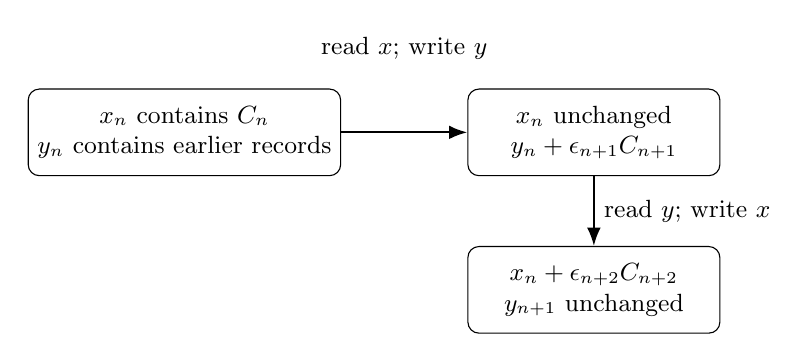
\begin{tikzpicture}[>=Latex,font=\small]
\node[draw,rounded corners,align=center,minimum width=3.2cm,minimum height=1.1cm]
 (a) at (0,0) {$x_n$ contains $C_n$\\$y_n$ contains earlier records};
\node[draw,rounded corners,align=center,minimum width=3.2cm,minimum height=1.1cm]
 (b) at (5.2,0) {$x_n$ unchanged\\$y_n+\epsilon_{n+1}C_{n+1}$};
\node[draw,rounded corners,align=center,minimum width=3.2cm,minimum height=1.1cm]
 (c) at (5.2,-2) {$x_n+\epsilon_{n+2}C_{n+2}$\\$y_{n+1}$ unchanged};
\draw[->,thick] (a)--node[above=8mm]{read $x$; write $y$}(b);
\draw[->,thick] (b)--node[right]{read $y$; write $x$}(c);
\end{tikzpicture}
\caption{Two successive slots, starting with even $n$. Every old record
remains present. The donor does not move during its slot, so its decoded
instruction stays constant while the new record is written. The signal
coordinate $z$ is omitted from the diagram.}
\label{fig:alternating}
\end{figure}

\subsection{A smooth decoder on every real donor value}
The positional tape representation is a generalized-shift encoding
\cite{Moore}. We now give the decoder on arbitrary real arguments,
so the field is defined independently of the distinguished execution.
Choose rational $m<a_P<b_P<1$ and define on $[0,1]$
\[
 P(v)=v-H\bigl((v-a_P)/(b_P-a_P)\bigr).
\]
Near zero this is $v$, and near one it is $v-1$; it therefore extends
to a smooth bounded $1$-periodic function, with all derivatives bounded.
It equals the fractional part whenever that fractional part belongs to
$[0,m]$.  For slot $n$, let the donor $D$ be $x$ when $n$ is even and
$y$ when $n$ is odd, and set
\begin{equation}
 C=P(b^{s_n}D),\qquad B=P(b^{s_n+1+K_n}D),\qquad
 A=P(b^{s_n+1}D)-b^{-K_n}B.
 \label{eq:alternating-read}
\end{equation}
At the intended donor these give $C_n,\eta_n,\xi_n$ respectively.
To verify this, every earlier donor block with index $j<n$ contributes
an integer after multiplication by $b^{s_n}$: its denominator is
$b^{s_j+1+2K_j}$, and
$s_n\geq s_{j+1}>s_j+1+2K_j$.  The remaining block is $C_n$.
Multiplication once more by $b$ removes the state digit.  Multiplication
by $b^{K_n}$ removes the first $K_n$ tape digits since
$b^{K_n}\xi_n$ is an integer, leaving the tail $\eta_n$.
All fractional parts used here lie in $[0,m]$, where $P$ is exact.
Subtraction then gives $A=\xi_n$.  This is the precise role of old-scale
divisibility in the alternating encoding.

Make a finite list of the normalized table branches, including its
freezing halting transitions, and split each left move by its left-top
symbol $\ell$. For a branch
$i:(q,a)\mapsto(p_i,b_i,d_i)$ put
\[
 \Psi_i(D)=\phi_q(C)\phi_a(B)
 \begin{cases}1,&d_i=0,1,\\\phi_\ell(A),&d_i=-1.\end{cases}
\]
Let $R=bB-g_a$ and define its tape update by
\begin{equation}
 (T_i^1,T_i^2)=
 \begin{cases}
 ((g_{b_i}+A)/b,R),&d_i=1,\\
 (A,(g_{b_i}+R)/b),&d_i=0,\\
 (bA-g_\ell,(g_\ell+(g_{b_i}+R)/b)/b),&d_i=-1.
 \end{cases}
 \label{eq:alternating-update}
\end{equation}
At an intended donor precisely the correct branch has weight one, and
all others vanish.  The displayed digit push and pop formulas give
$\xi_{n+1},\eta_{n+1}$, which fit in $K_{n+1}$ places.  Define, on
all real donor arguments,
\begin{align}
 L_n(D)&=\frac{\epsilon_{n+1}}b
    \sum_i\Psi_i(D)
       \bigl(g_{p_i}+T_i^1+b^{-K_{n+1}}T_i^2\bigr),
       \label{eq:alternating-write}\\
 E_n(D)&=\epsilon_n-\epsilon_{n+1}
       +2\epsilon_{n+1}\sum_{q\in H_Q}\phi_q(C).
       \label{eq:alternating-signal}
\end{align}
Thus $L_n(D)=\epsilon_{n+1}C_{n+1}$ on the intended donor.
The field retains all old records, so the branches need no disjoint
images and no reversible-table preprocessing.

\subsection{Keeping the donor stationary during the write}
Choose one fixed compact cutoff $\chi$ equal to one on a neighborhood
of $[0,1]^2\times[-1,1]$ in $(x,y,z)$ coordinates, again using rational
rescalings of the effective cutoffs so that every derivative has an
effective bound. In slot
$[1+n,2+n]$ prescribe $U=\theta'(t-1-n)V_n$, where
\begin{equation}
 V_n=
 \begin{cases}
 \operatorname{curl}(\chi(zL_n(x)-yE_n(x)),0,0),&n\text{ even},\\
 \operatorname{curl}(0,\chi(xE_n(y)-zL_n(y)),0),&n\text{ odd}.
 \end{cases}
 \label{eq:alternating-curls}
\end{equation}
On the plateau these velocities are respectively $(0,L_n,E_n)$ and
$(L_n,0,E_n)$.  In particular the donor is stationary throughout its
slot. During initialization, for $0\leq t\leq1$, set
\[
 d=(\epsilon_0C_0,0,1-\epsilon_0),\qquad
 U(t,x,y,z)=\theta'(t)\operatorname{curl}
 \left[\frac12\chi(x,y,z)\bigl(d\times(x,y,z)\bigr)\right].
\]
On the plateau this equals $\theta'(t)d$, so the particle follows
$(0,0,-1)+\theta(t)d$. This whole segment lies in the plateau.
Only the initial code $C_0$ is supplied to the field.

We verify the trajectory before using it for observation.  Initialization
ends at $(\epsilon_0C_0,0,-\epsilon_0)$.  If the memories at the
start of slot $n$ are \eqref{eq:alternating-history}, the
stationary donor gives the values in \eqref{eq:alternating-read}.
With progress $\theta(t-1-n)$, the other memory acquires $L_n(D)$
and the signal acquires $E_n(D)$.  This proves the next memory identity.
All proposed paths remain on the plateau: the two memories are between
zero and $\sum_j\epsilon_j$, and
\[
 \sum_{j\geq0}\epsilon_j\leq2\epsilon_0<1/4.
\]
Here $s_{j+1}-s_j\geq1$ and $b\geq4$ already give a geometric
majorant; the stated constant two is more than sufficient.  The signal
starts at $-\epsilon_0$, and each increment lies between zero and
$\epsilon_n+\epsilon_{n+1}$.  Its total displacement is less than
$2\sum_j\epsilon_j<1/2$.  Hence $|z|<1$ on all slots, even after
halting.  The proposed curves genuinely solve the cutoff field, and
ODE uniqueness identifies them with the material trajectory.

Before the first slot whose current state is halting, the signal is
$-\epsilon_n$ at the slot's start and interpolates monotonically to
$-\epsilon_{n+1}$, remaining strictly negative.  In the first halting
slot it instead ends at $+\epsilon_{n+1}$.  This also covers an initially
halting machine, which is detected in the first post-loading slot.
Loading stays negative.  Thus $z=X_1>0$ occurs exactly when the machine
halts, with no intermediate false positive.

\subsection{Derivative bounds and effective evaluation}
The particle correspondence has been proved for every real time. It
remains to prove that the field defining it has the claimed rapid bounds.  The
functions $C,A,B$ in \eqref{eq:alternating-read} are uniformly
bounded.  Applying the chain and product rules through spatial order
$r$ gives
\[
 \left\|L_n/\epsilon_{n+1}\right\|_{C^r}
 +\left\|\sum_{q\in H_Q}\phi_q(C)\right\|_{C^r}
 \leq C_r b^{r(s_n+1+K_n)}.
\]
Constants depend on the fixed table, base, and smooth functions, but not
on $n$.  The factors $b^{-K_n}$ and $b^{-K_{n+1}}$ are at most one;
there are only finitely many branches.  Accounting for one derivative
in the curl and for the fixed cutoff yields
\begin{equation}
 \|V_n\|_{C^r}
 \leq C_r'\left(b^{-s_n}
      +b^{-s_{n+1}+(r+1)(s_n+1+K_n)}\right).
 \label{eq:alternating-estimate}
\end{equation}
For each fixed $r$, the second term is at most $b^{-s_n}$ for all
sufficiently large $n$, because $s_{n+1}/s_n=2^{2n+7}$ and
$K_n+1<s_n$.  Temporal derivatives only differentiate the fixed
clock pulse, and the zero collars give smooth gluing.  The right side
therefore tends to zero faster than every inverse power of $1+n$ for
each fixed mixed order.  Early slots and loading have finite individual
bounds.  These facts prove all the rapid mixed bounds for $U$.

For $f=\mathcal R_\nu[U]$, the linear terms require one additional
time derivative or two additional spatial derivatives.  Each derivative
of the quadratic term is a finite sum of products of mixed derivatives
of $U$, one with an additional spatial derivative.  The already proved
estimates bound every such factor; one factor may carry any requested
temporal weight and the other is bounded.  Consequently $f$ has every
rapid mixed bound.  Fixed compact support turns a temporal weight into
the full weight $(1+t+|X|)^J$ in
\eqref{eq:alternating-schwartz}.  The fixed support gives all Sobolev conditions in
\eqref{eq:energy-class}. Lemma~\ref{lem:realization} supplies
uniqueness and the global material flow.

For a finite slot index all scales, the fixed branch list, and all
coefficients are effective.  A coarse enclosing time interval selects
finitely many candidate slots; zero collars make evaluation consistent
where such choices overlap.  The periodic function $P$ can be evaluated
by finitely many neighboring integer translates, or by its affine
formula across an integer, without a discontinuous fractional-part
test.  Flat cutoff bounds and finite differentiation give arbitrary
rational-error evaluation of the field, the force, and every derivative.
Bounds for any fixed finite set of orders are obtained from a finite
initial range plus the explicit tail inequality in
\eqref{eq:alternating-estimate}.  Only $C_0$ is computed from
the input orbit; subsequent slot functions perform one local table
update on their spatial donor arguments.  Physical slots have unit
length and no finite accumulation time. This proves
Theorem~\ref{thm:alternating}.

\section{Periodic lattice memory on the torus}
\label{sec:lattice}

We now store successive configurations in a single torus coordinate.
The earlier records remain in that coordinate, but a residue calculation
removes them when the next transition is read.  A second coordinate
records whether the current state is halting.  Both the new record and
the halting signal become much smaller at each step.  This separation of
scales will make every derivative of the velocity and force decay faster
than every inverse power of time. The positional stack operations belong
to the generalized-shift approach \cite{Moore}; the residue arithmetic
and smooth realization are proved below.

The planar motion used for this purpose need not preserve area.  We
first construct and verify that motion.  A third component will then
cancel its divergence while leaving the coding plane invariant.

\begin{theorem}[Periodic lattice memory]\label{thm:lattice}
Fix a computable viscosity $\nu>0$.  A finite deterministic machine and
a finite input effectively determine a smooth force $g$ on the unit
flat torus $\T^3=(\R/\mathbb Z)^3$ with zero spatial mean.  The
Navier--Stokes equations with force $g$ and zero initial velocity have
a smooth solution $(U,0)$ with zero spatial mean.  Its particle from
\[
 a_*=(1/4,1/2,1/2)
\]
enters the fixed open set
\[
 O=\{x\in\T^3:1/2<x_1<1\pmod 1\}
\]
at some finite time if and only if the machine halts on that input.
For every pair of nonnegative integers $r,J$ and every spatial
multi-index $\alpha$, there is an effective constant $C_{r,\alpha,J}$
such that
\begin{equation}\label{eq:lattice-rapid}
 \|\partial_t^r\partial_x^\alpha U(t)\|_\infty
 +\|\partial_t^r\partial_x^\alpha g(t)\|_\infty
 \le C_{r,\alpha,J}(1+t)^{-J},\qquad t\ge0.
\end{equation}
There is also an effective smooth mean-zero solenoidal force $f$
with the same bounds and exactly the same velocity and material event.
It is $f=g-\nabla\phi$, with pressure $-\phi$, where $\phi$ is the
mean-zero periodic solution of $\Delta\phi=\operatorname{div}g$.

For either force, uniqueness holds among periodic classical solutions
for which the velocity, its time derivative and its spatial derivatives
through order two, and the pressure and its spatial gradient, are
continuous on every $[0,T]\times\T^3$.  Pressure is normalized to have
zero spatial mean.
\end{theorem}

\subsection{Reading a configuration from an integer residue}

Normalize a missing instruction by entering a fresh halting state without
moving or changing the scanned symbol. To retain absolute
tape position as well as the contents relative to the head, add a
read-only bit track with a unique marked bit at the initial origin.
Transitions preserve the bit and ignore it when choosing an instruction.
The resulting alphabet is denoted by $\Gamma$, its all-blank symbol by
$\square$, its state set by $Q$, and its finite initial word by $\omega$.
The word contains the marked origin even when the original input is
empty.  This modification preserves halting.

Choose $b=\max(2,|\Gamma|,|Q|)$.  Give the symbols distinct digits in
$\{0,\ldots,b-1\}$, assigning zero to $\square$, and number the states
from zero.  After $n$ transitions, put
\[
 d_n=|\omega|+1+2n,\qquad p_n=2d_n+1,\qquad P_n=b^{p_n}.
\]
The nearest $d_n$ cells to the left of the head form a stack with
integer code $L$; the nearest $d_n$ cells starting at the head form a
stack with code $R$.  In each stack the nearest cell is the least
significant base-$b$ digit.  All cells outside these two stacks are
blank: a head travels at most one cell per transition, whereas the
available width grows by two.  If the state number is $s$, the complete
configuration therefore has the code
\begin{equation}\label{eq:lattice-code}
 c_n=L+b^{d_n}R+b^{2d_n}s,\qquad 0\le c_n<P_n.
\end{equation}
The slot number $n$ specifies the stack width.  The origin bit determines
the head's absolute position, so the code loses no tape information.

We must prescribe the field at every spatial address, rather than only
at addresses visited by this computation.  For an arbitrary integer
$j$, let $[j]_q$ denote its least nonnegative residue modulo the positive
integer $q$.  Extract
\[
 \begin{split}
 c&=[j]_{P_n},\\
 L&=[c]_{b^{d_n}},\qquad
 R=\bigl[\lfloor c/b^{d_n}\rfloor\bigr]_{b^{d_n}},\\
 s&=\lfloor c/b^{2d_n}\rfloor,\qquad
 l=[L]_b,\quad a=[R]_b.
 \end{split}
\]
Define $h_n(j)=1$ if $s$ is a halting-state index, and $h_n(j)=0$
otherwise.  If $s$ is a valid nonhalting state and $a$ a valid symbol,
look up the single instruction $(s,a)\mapsto(s',a',m)$, where
$m\in\{-1,0,1\}$.  Set
\begin{equation}\label{eq:lattice-transition}
 \begin{split}
 (L',R')&=
 \begin{cases}
 (a'+bL,(R-a)/b),&m=1,\\
 ((L-l)/b,l+ba'+b(R-a)),&m=-1,\\
 (L,R-a+a'),&m=0,
 \end{cases}\\
 F_n(j)&=L'+b^{d_{n+1}}R'+b^{2d_{n+1}}s'.
 \end{split}
\end{equation}
In every other case define $F_n(j)=0$.  Digits away from the scanned
cell need not be checked for membership in the alphabet.

\begin{lemma}\label{lem:lattice-address}
The functions $F_n,h_n$ on $\mathbb Z$ are $P_n$-periodic,
$h_n\in\{0,1\}$, and $0\le F_n<P_{n+1}$ at every address.
If $c_n$ is a true nonhalting configuration and
$j\equiv c_n\pmod {P_n}$, then $F_n(j)=c_{n+1}$.
\end{lemma}
\begin{proof}
All extracted data depend only on $[j]_{P_n}$.  In each nonzero branch,
$0\le L',R'<b^{d_n+1}$.  For the left move, the only less immediate
bound follows from
\[
 R-a\le b^{d_n}-b,\qquad l,a'\le b-1,
\]
which give $l+ba'+b(R-a)\le b^{d_n+1}-1$.  The right and stationary
branches satisfy the same bounds directly.  Since $d_{n+1}=d_n+2$
and $0\le s'<b$, the output fits in the three fields of the next code.
The formulas are precisely the stack operations for a tape transition.
In particular, after a left move the new right stack consists of the
old left top, the symbol just written, and the old right tail.  This is
$l+ba'+b(R-a)$; the last term has two digit shifts because $R-a$
already contains one factor of $b$.  The two new blank places suffice
for every branch.
\end{proof}

\subsection{Scales that retain old records without reading them}

Suppose a real coordinate stores a partial history as
$y_*+\sum_{k=0}^n\epsilon_kc_k$, with $y_*=1/2$.
To recover $c_n$, we want every earlier summand, after division by
$\epsilon_n$, to be an integer multiple of $P_n$.  We also want the
next displacement to be much smaller than $\epsilon_n$, so a smooth
selector will read the same integer throughout that displacement.
The following explicit scales meet both requirements:
\begin{equation}\label{eq:lattice-scales}
 K_n=(p_0+10)2^{n(n+1)},\qquad
 \epsilon_n=b^{-K_n},\qquad
 \beta_0=1/4,\quad \beta_n=\epsilon_n\quad(n\ge1).
\end{equation}
The numbers $\beta_n$ give the distance of a nonhalting signal from
the boundary $x_1=1/2$. The separate choice $\beta_0=1/4$ fixes the
initial first coordinate at $1/4$, independently of the input; later
distances use the shrinking memory scales. Its contribution to the
first transition is a single finite-time term in the decay estimates.

\begin{lemma}\label{lem:lattice-scales}
For $n\ge0$,
\begin{align}
 P_n&\mid\epsilon_n^{-1},&
 P_n&\mid\epsilon_k/\epsilon_n\quad(0\le k<n),
 \label{eq:lattice-divisibility}\\
 P_{n+1}\epsilon_{n+1}
 &\le\epsilon_n^{\,2^{2n+2}-1}
 \le\epsilon_n^3<\epsilon_n/4.
 \label{eq:lattice-plateau-bound}
\end{align}
Moreover, $\beta_n$ decreases strictly and $\epsilon_n\le2^{-n}$.
\end{lemma}
\begin{proof}
Here $p_n=p_0+4n$ and $K_{n+1}=2^{2n+2}K_n$.
Induction gives $K_n\ge p_{n+1}$, starting with
$K_0=p_0+10\ge p_0+4$.  Thus $K_n\ge p_n$ and, for $k<n$,
\[
 K_n-K_k\ge K_n-K_{n-1}\ge3K_{n-1}\ge p_n.
\]
These inequalities prove the two divisibilities, since all quantities
are powers of the same integer $b$.  Also
\[
 b^{p_{n+1}-K_{n+1}}
 \le b^{K_n-2^{2n+2}K_n}
 =\epsilon_n^{\,2^{2n+2}-1}.
\]
The remaining assertions follow from $b\ge2$, $K_0\ge13$ and the
strict growth of $K_n$.
\end{proof}

We have now specified the finite rule table and the scale arithmetic.
The next step makes the residue calculation into a smooth field whose
actual particle follows the whole stored history.

\subsection{Smooth selectors and the complete particle path}

Fix an effective smooth nondecreasing function $\sigma$ with
$\sigma(t)=0$ for $t\le1/3$ and $\sigma(t)=1$ for $t\ge2/3$.
Take $\sigma(t)=H(3t-1)$ with the function $H$ fixed in
Section~\ref{sec:analytic}.
Choose an effective smooth bump $\psi$ that is one on $[-1/4,1/4]$
and zero outside $[-3/8,3/8]$.  Products of translates and rescalings
of $H$ supply such a bump.  These functions and their derivatives have
effective bounds; flatness at the endpoints follows from the
exponential factor in $\rho$.

For $j\in\mathbb Z$, define a bump centered at the $j$th point of
the scale-$n$ lattice by
\[
 J_{n,j}(y)=\psi\bigl((y-y_*)/\epsilon_n-j\bigr).
\]
Their supports are pairwise disjoint.  In planar coordinates
$\xi=(\xi_1,\xi_2)$, prescribe the loading field and the $n$th
transition field by
\begin{align}
 v_{\rm in}(t,\xi)&=\sigma'(t)(0,\epsilon_0c_0),
 \label{eq:lattice-loader}\\
 v_n(t,\xi)&=\sigma'(t-1-n)
 \begin{pmatrix}
  \beta_n-\beta_{n+1}
     +2\beta_{n+1}\displaystyle\sum_{j\in\mathbb Z}h_n(j)J_{n,j}(\xi_2)\\
  \epsilon_{n+1}\displaystyle\sum_{j\in\mathbb Z}F_n(j)J_{n,j}(\xi_2)
 \end{pmatrix},
 \label{eq:lattice-slot}\\
 v&=v_{\rm in}+\sum_{n\ge0}v_n.
 \label{eq:lattice-planar-field}
\end{align}
The field is independent of $\xi_1$.  Translation of $\xi_2$ by
one shifts the lattice index by $\epsilon_n^{-1}$, a multiple of
$P_n$ by Lemma~\ref{lem:lattice-scales}.  The coefficients therefore
repeat, and $v$ is a field on $\T^2$.  Only the loader acts during
$[0,1]$, and only $v_n$ acts during $[1+n,2+n]$.  The fixed zero
collars of the pulses make their sum smooth, including at every slot
boundary and at time zero.

Let $Y(t)$ be the real-coordinate lift of its particle starting at
$(1/4,y_*)$.  The loader leaves the first coordinate unchanged and
ends at
\[
 Y(1)=(1/4,y_*+\epsilon_0c_0).
\]
We claim that, at $t_n=1+n$ and up to the first halting configuration,
\begin{equation}\label{eq:lattice-history}
 Y_1(t_n)=1/2-\beta_n,\qquad
 Y_2(t_n)=y_*+\sum_{k=0}^n\epsilon_kc_k.
\end{equation}
The claim holds for $n=0$.  Assuming it at $n$, put
\[
 j_*=(Y_2(t_n)-y_*)/\epsilon_n.
\]
This is an integer, and \eqref{eq:lattice-divisibility} gives
$j_*\equiv c_n\pmod {P_n}$.  Changing the lift of $Y_2$ by an
integer changes $j_*$ by a multiple of $P_n$, so the decoded instruction
is intrinsic to the torus.

Throughout this slot the actual trajectory is
\begin{align}
 Y_2(t_n+\tau)&=Y_2(t_n)+\sigma(\tau)\epsilon_{n+1}F_n(j_*),
 \label{eq:lattice-path-y}\\
 Y_1(t_n+\tau)&=Y_1(t_n)+\sigma(\tau)
  \bigl(\beta_n-\beta_{n+1}+2\beta_{n+1}h_n(j_*)\bigr),
 \quad 0\le\tau\le1.
 \label{eq:lattice-path-x}
\end{align}
Indeed, Lemma~\ref{lem:lattice-address} and
\eqref{eq:lattice-plateau-bound} bound the second-coordinate
displacement by $\epsilon_n/4$.  The proposed curve stays on the
plateau $J_{n,j_*}=1$, where every other bump vanishes.  Differentiating
\eqref{eq:lattice-path-y}--\eqref{eq:lattice-path-x} therefore gives
exactly \eqref{eq:lattice-slot}.  Spatial smoothness and ODE uniqueness
identify it with the actual particle.

At a nonhalting configuration, Lemma~\ref{lem:lattice-address} gives
$F_n(j_*)=c_{n+1}$ and $h_n(j_*)=0$.  The endpoint is thus the next
history in \eqref{eq:lattice-history}.  Throughout that slot the first
coordinate lies between $1/2-\beta_n$ and $1/2-\beta_{n+1}$, both
strictly below $1/2$.  At a halting configuration $h_n(j_*)=1$, and
the first-coordinate endpoint is instead
\[
 Y_1(t_n+1)=1/2+\beta_{n+1}\in(1/2,1).
\]
This also handles an initially halted input, whose signal appears in
the first slot after loading.  There is no first-coordinate wrap before
the first detection.  Consequently the open event has the required
equivalence at all real times, not just at integer endpoints.

\subsection{Rapid bounds and the incompressible lift}

The stored history grows, but neither its length nor the number of
lattice cells enters a derivative bound.  At each spatial point at most
one bump in \eqref{eq:lattice-slot} is nonzero.  For $|\alpha|=k$,
all time orders $r$, and $n\ge0$, the coefficient bounds give
\begin{equation}\label{eq:lattice-slot-bound}
 \|\partial_t^r\partial_\xi^\alpha v_n\|_\infty
 \le C_{r,k}\left(\mathbf 1_{k=0}\beta_n
       +P_{n+1}\epsilon_{n+1}\epsilon_n^{-k}\right).
\end{equation}
The constant drift disappears after a spatial derivative; each derivative
of a bump costs one factor of $\epsilon_n^{-1}$.  For
$n\ge\max(1,k)$, \eqref{eq:lattice-plateau-bound} bounds the
right-hand side by $C'_{r,k}\epsilon_n$.  Since
$\epsilon_n\le2^{-n}$ and $1+t\le n+3$ on the $n$th slot,
every polynomial time weight is bounded.  The finitely many earlier
slots and the loader contribute finite effective constants.  Thus $v$
satisfies all the mixed rapid bounds in \eqref{eq:lattice-rapid}.

Choose an effective smooth periodic function $\eta$ on $\T$ with
$\eta(1/2)=0$ and $\eta'(1/2)=1$.  One explicit choice is
$(z-1/2)$ times a smooth cutoff supported in
$(1/2-3/16,1/2+3/16)$ and equal to one near $1/2$, extended periodically.
Define on $\T^3$
\begin{equation}\label{eq:lattice-lift}
 U(t,\xi,z)=
 \bigl(\eta'(z)v_1(t,\xi),\eta'(z)v_2(t,\xi),
       -\eta(z)\operatorname{div}_\xi v(t,\xi)\bigr).
\end{equation}
The two divergence terms cancel.  The first two components have zero
mean because $\int_\T\eta'=0$, and the third has zero mean because
$\int_{\T^2}\operatorname{div}_\xi v=0$.  On the plane $z=1/2$,
the velocity is exactly $(v,0)$, so the plane is invariant and the
particle from $a_*$ is $(Y(t),1/2)$ modulo integers.  This proves that
the fluid lift preserves the event already verified.

The lift costs at most one planar derivative of $v$.  Consequently $U$
obeys all the rapid estimates, is zero initially, and has bounded
gradient on each finite time interval.  Put
\begin{equation}\label{eq:lattice-residual}
 g=\partial_tU+(U\cdot\nabla)U-\nu\Delta U.
\end{equation}
This is the residual-realization construction of
Lemma~\ref{lem:realization}: a prescribed smooth divergence-free
velocity from rest solves the forced equation with this force and
pressure zero.  Here $g$ has zero mean, since its time-derivative
and Laplacian terms integrate to zero and
$(U\cdot\nabla)U=\operatorname{div}(U\otimes U)$.
Product differentiation proves every rapid bound for $g$.  More
explicitly, a derivative of spatial order $k$ of the residual uses
planar derivatives through order $k+3$ and one additional time
derivative, all supplied by \eqref{eq:lattice-slot-bound}.

The field $U$ satisfies the periodic classical hypotheses of
Lemma~\ref{lem:realization}. That lemma gives the stated uniqueness
class, the mean-zero pressure normalization, and the unique global
material flow.

\subsection{Effective evaluation and solenoidal forcing}

The formulas specify all instructions without generating the distinguished
execution.  Given a computable time, a rational enclosure selects
finitely many possible pulse slots.  Within a selected slot, enclose
a real lift of the second coordinate in a rational interval of length
at most $\epsilon_n/2$.  Include every lattice center whose bump
support meets that interval.  The number of candidates is uniformly
bounded, and every omitted term vanishes.  Summing these candidates
avoids deciding whether a computable real lies exactly on a cell
boundary.  Each coefficient requires integer arithmetic and one lookup
in the finite transition table.  Only the loading code $c_0$ uses the
input contents; the later fields use the table and the transformed
input length.

The cutoff formulas have effective derivative bounds, and
\eqref{eq:lattice-slot-bound} supplies an effective tail estimate.
For any fixed $J$, an upper bound on $(n+3)^J2^{-n}$ is computable,
for example by checking finitely many terms until its successive ratio
is bounded by a fixed number below one.  Values of the fields, residual,
and every requested derivative can therefore be evaluated to arbitrary
rational error.  If $\nu$ is an arbitrary fixed positive real instead,
the same algebraic formulas hold, with numerical evaluation relative
to that parameter.

Finally apply Lemma~\ref{lem:projection} to $g$. We have proved its
zero spatial mean and effective estimates at every mixed order and
every temporal weight. Thus the mean-zero solution of
$\Delta\phi=\operatorname{div}g$ gives the effective solenoidal force
\[
 f=g-\nabla\phi,\qquad p=-\phi.
\]
Equation~\eqref{eq:projection} specifies its coefficients, and the
weighted conclusion of the lemma gives \eqref{eq:lattice-rapid}.
The pressure sign preserves $-\nabla p+f=g$, hence precisely the
same velocity and particle event. A competitor for $f$ with pressure
$q$ becomes a competitor for $g$ with pressure $q+\phi$, in the same
normalized classical class. This also proves the projected uniqueness
and completes Theorem~\ref{thm:lattice}.



\section{What the detector decides}\label{sec:consequences}

The constructions give four fixed experiments: the addressed Euclidean
field, its torus image, the alternating Euclidean field, and the periodic
lattice field. In each case the domain, particle label, detector and
viscosity are fixed before the machine and word are supplied.
The shrinking scales depend effectively on finite input data, and every
transition occupies an entire unit time slot.

\begin{corollary}\label{cor:undecidable}
For each of these four experiments, no algorithm decides the particle
event for every force program produced by its construction. This remains
true for the solenoidal mean-zero versions of the two torus experiments.
\end{corollary}
\begin{proof}
Composing such an algorithm with the finite compiler would decide
halting for arbitrary machines and words. This would decide Turing's
symbol-printing problem \cite[Section~8]{Turing}: simulate the given
machine, halt when the designated symbol is printed, and continue forever
if the machine stops without printing it. Turing proves that no such
decision procedure exists.
\end{proof}

The exact observers also describe the limitation. In the addressed
construction the nonhalting first coordinate is exactly $-1$ after
loading, on the boundary of its open detector; a halt in slot $n$ moves
it by $-b_n$. Its torus image has boundary $3/8$ and signal $b_n/8$.
The alternating signal approaches zero from below, while the lattice
signal approaches $1/2$ from below. In both cases the first halting slot
crosses that boundary by a positive amount depending on its index.
Those amounts tend to zero. Consequently these proofs give no positive
lower bound on the separation required for a uniform finite-precision
test, and no assertion of robustness under a fixed measurement or field
perturbation. This qualification concerns the constructions proved here;
it does not contradict robust tape-bounded fluid simulations.

There is no conflict between rapid decay and invertibility of the flow.
Earlier records remain in the particle coordinates, even when a residue
or a smooth periodic decoder ignores them. There is also no accumulation
of infinitely many instructions at a finite physical time. What decreases
is the distance needed to write the next record and to signal a halt.

\begin{thebibliography}{10}
\bibitem{Bennett} C.~H. Bennett, Logical reversibility of computation,
\emph{IBM J. Res. Develop.} \textbf{17} (1973), 525--532.
\href{https://doi.org/10.1147/rd.176.0525}{\nolinkurl{doi:10.1147/rd.176.0525}}.

\bibitem{CMPBeltrami}
R. Cardona, E. Miranda and D. Peralta-Salas,
Computability and Beltrami fields in Euclidean space,
\emph{J. Math. Pures Appl.} \textbf{169} (2023), 50--81.
\href{https://doi.org/10.1016/j.matpur.2022.11.007}{\nolinkurl{doi:10.1016/j.matpur.2022.11.007}}.
Theorem locators refer to \href{https://arxiv.org/abs/2111.03559v3}{arXiv:2111.03559v3}.

\bibitem{CMPP} R. Cardona, E. Miranda, D. Peralta-Salas and F. Presas,
Constructing Turing complete Euler flows in dimension 3,
\emph{Proc. Natl. Acad. Sci. USA} \textbf{118} (2021), e2026818118.
\href{https://doi.org/10.1073/pnas.2026818118}{\nolinkurl{doi:10.1073/pnas.2026818118}}.

\bibitem{DGMP}
S. Dyhr, \'A. Gonz\'alez-Prieto, E. Miranda and D. Peralta-Salas,
Turing complete Navier--Stokes steady states via cosymplectic geometry,
\emph{PNAS Nexus} \textbf{5} (2026), no.~5, pgag131.
\href{https://doi.org/10.1093/pnasnexus/pgag131}{\nolinkurl{doi:10.1093/pnasnexus/pgag131}}.

\bibitem{Landauer} R. Landauer, Irreversibility and heat generation in
the computing process, \emph{IBM J. Res. Develop.} \textbf{5} (1961),
183--191.
\href{https://doi.org/10.1147/rd.53.0183}{\nolinkurl{doi:10.1147/rd.53.0183}}.

\bibitem{Leray} J. Leray, Sur le mouvement d'un liquide visqueux
emplissant l'espace, \emph{Acta Math.} \textbf{63} (1934), 193--248.
\href{https://doi.org/10.1007/BF02547354}{\nolinkurl{doi:10.1007/BF02547354}}.

\bibitem{Moore1990} C. Moore, Unpredictability and undecidability in
dynamical systems, \emph{Phys. Rev. Lett.} \textbf{64} (1990), 2354--2357.
\href{https://doi.org/10.1103/PhysRevLett.64.2354}{\nolinkurl{doi:10.1103/PhysRevLett.64.2354}}.

\bibitem{Moore} C. Moore, Generalized shifts: unpredictability and
undecidability in dynamical systems, \emph{Nonlinearity} \textbf{4}
(1991), 199--230.
\href{https://doi.org/10.1088/0951-7715/4/2/002}{\nolinkurl{doi:10.1088/0951-7715/4/2/002}}.

\bibitem{CompanionA}
OpenAI, A Fixed Particle Test for Computation in a Forced Viscous Flow,
OpenAI Math Release preprint
\href{https://github.com/openai/math/blob/main/preprints/A-Fixed-Particle-Test-for-Computation-in-a-Forced-Viscous-Flow-September-27-2026/manuscript.pdf}{OAI:A-Fixed-Particle-Test-for-Computation-in-a-Forced-Viscous-Flow-September-27-2026},
2026.

\bibitem{Turing} A.~M. Turing, On computable numbers, with an application
to the Entscheidungsproblem, \emph{Proc. London Math. Soc.} (2)
\textbf{42} (1936--1937), 230--265.
\href{https://doi.org/10.1112/plms/s2-42.1.230}{\nolinkurl{doi:10.1112/plms/s2-42.1.230}}.
\end{thebibliography}

\end{document}
